\documentclass[main.tex]{subfiles}
\begin{document}

\section{Sheet 2}

\subsection{Constant acceleration}

We are given the position as a function of time, 
\begin{equation}
  x(t) = \frac{\sqrt{1 + \kappa^2 t^2} -1 }{\kappa }\,,
\end{equation}
%
and we can directly compute its derivative
%
\begin{equation}
  v(t) = \dv{x}{t} =
  \frac{\kappa t}{\sqrt{\kappa^2 t^2  + 1} }\,.
\end{equation}

It is clear from the expression that \(\abs{v} < 1\) for all times, while \(v\) approaches 1 at positive temporal infinity and \(-1\) at negative temporal infinity.

\begin{figure}[h]
    \centering
    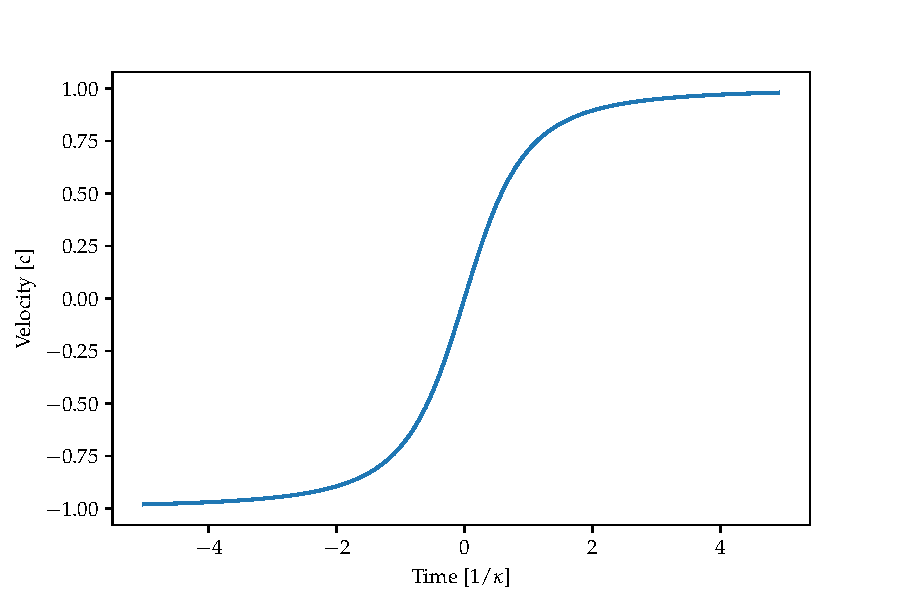
\includegraphics[width=\textwidth]{figures/velocity.pdf}
    \caption{Velocity as a function of coordinate time \(t\)}
    \label{fig:velocity-constant-acceleration}
\end{figure}

The Lorentz factor \(\gamma \) is given by
%
\begin{equation}
  \gamma = \frac{1}{\sqrt{1-v^2}}
  = \frac{1}{\sqrt{1 - \frac{\kappa^{2} t^{2}}{\kappa^{2} t^{2} + 1} }}
  = \sqrt{\kappa^2 t^2 + 1} \,,
\end{equation}
%
therefore the four-velocity is given by:
%
\begin{equation}
  u^{\mu } =
  \begin{bmatrix}
  \gamma  \\
  \gamma v \\
  0 \\
  0
  \end{bmatrix}
  =
  \begin{bmatrix}
    \sqrt{\kappa^2 t^2 + 1}  \\
    \kappa t \\
    0 \\
    0
  \end{bmatrix}\,.
\end{equation}

The relation between coordinate and proper time is given by the definition of the first component of the four-velocity: \(u^{0} = \dv*{t}{\tau} = \gamma \), therefore \(\dd{\tau } = \dd{t} / \gamma \).
Integrating this relation we get:
%
\begin{equation}
    \tau = \int \dd{\tau } 
    = \int \frac{\dd[]{t} }{\gamma }
    = \displaystyle \frac{\operatorname{arcsinh}{\left(\kappa t \right)}}{\kappa}\,,
\end{equation}
%
where the constant of integration is selected by imposing \(t = 0 \iff \tau = 0\).
Notice that, as we would expect, when expanding up to second order near \(t = \tau = 0 \) we have \(t \sim \tau \), since in that region the velocity is much less than unity.

The inverse relation is given by \(t = \sinh (\kappa \tau ) / \kappa \). Using this, we can write:
%
\begin{equation}
  x (t(\tau ))  =\frac{\cosh{\left(\kappa \tau \right)} - 1}{\kappa}\,.
\end{equation}

Now, we wish to compute the four-


\end{document}